\section{Industrial Context and Motivation}
\label{sec:background}

\subsection{Image Capture Reliability}
\label{sec:release-process}

The Samsung camera software is a privileged system application whose image-capture workflow spans multiple system-level components across the Android software stack.
Consequently, capture failures discovered late in the release cycle may require firmware-level changes involving cross-component coordination and extensive revalidation.
To detect capture failures early, the latest development builds are automatically tested each day across camera workflows, device models, and OS versions.
In addition to this daily testing, the camera-validation team and development engineers periodically stress-test the latest builds to identify timing- and memory-related failures, diagnose their root causes, and verify fixes.
Together, these activities form the core validation process for capture reliability.

A key reliability criterion in this validation process is a fixed internal deadline, referred to as the \emph{Capture Timeout}.
For each capture request, the timeout clock starts when the framework accepts the request, and the draft sequence must produce an initial user-visible image, called the \emph{draft image}, before the deadline.
If the draft sequence fails to produce the draft image within this deadline, the application intentionally crashes to make the violation observable.
Identifying and resolving such violations is therefore an important part of Samsung's pre-release validation process.

% Notes: docs/exhibits.md#fig_draft_final_gap
\begin{figure}[!ht]
  \centering
  \setlength{\tabcolsep}{1pt}%
  % All views are the same 1:1 frame (1080 bp source);
  % the zoom box keeps the source region x 162--702, y 695--875 bp from the bottom.
  % TODO: Replace the middle panel and its crop with the actual draft image
  % produced by lightweight multi-frame composition. Both temporarily reuse
  % fig_draft_final_gap_final.jpg; the caption explicitly marks this placeholder.
  \begin{tabular}{@{}ccc@{}}
    \begin{tikzpicture}
      \node[inner sep=0, anchor=south west] (im) at (0,0)
        {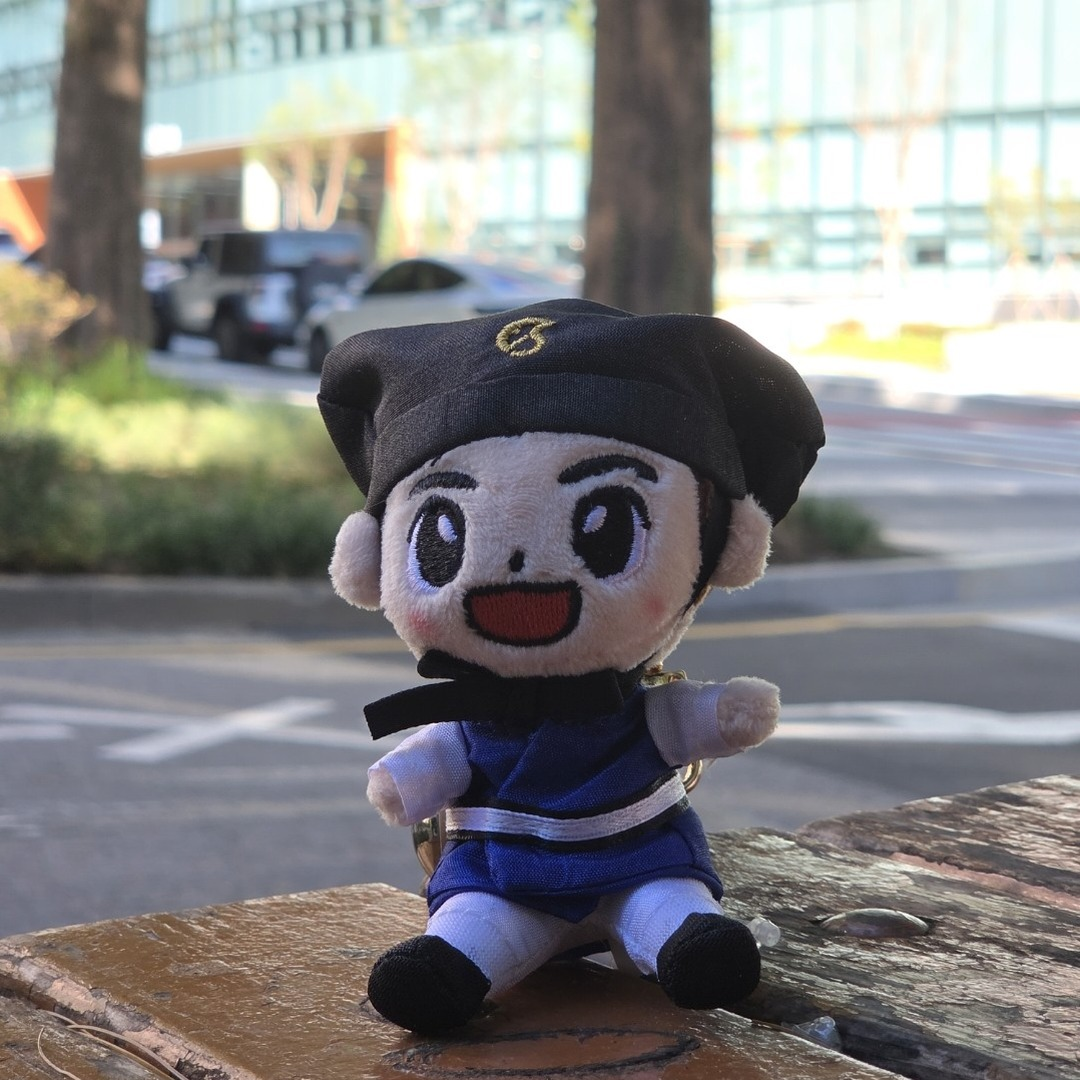
\includegraphics[width=0.325\columnwidth]{figures/fig_draft_final_gap_draft.jpg}};
      \begin{scope}[x={(im.south east)}, y={(im.north west)}]
        \draw[orange, line width=0.8pt] (0.15,0.6435) rectangle (0.65,0.8102);
      \end{scope}
    \end{tikzpicture} &
    \begin{tikzpicture}
      \node[inner sep=0, anchor=south west] (im) at (0,0)
        {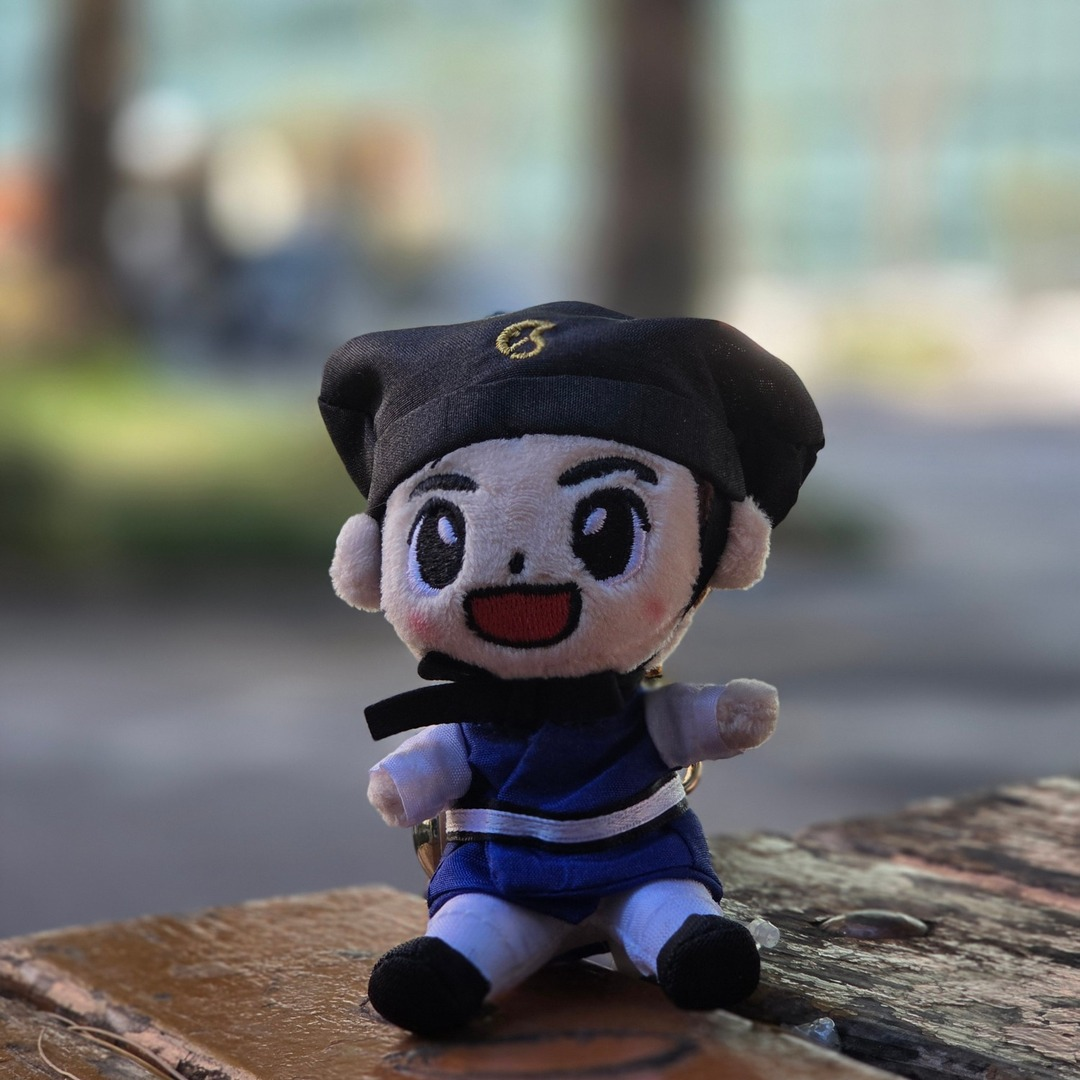
\includegraphics[width=0.325\columnwidth]{figures/fig_draft_final_gap_final.jpg}};
      \begin{scope}[x={(im.south east)}, y={(im.north west)}]
        \draw[orange, line width=0.8pt] (0.15,0.6435) rectangle (0.65,0.8102);
      \end{scope}
    \end{tikzpicture} &
    \begin{tikzpicture}
      \node[inner sep=0, anchor=south west] (im) at (0,0)
        {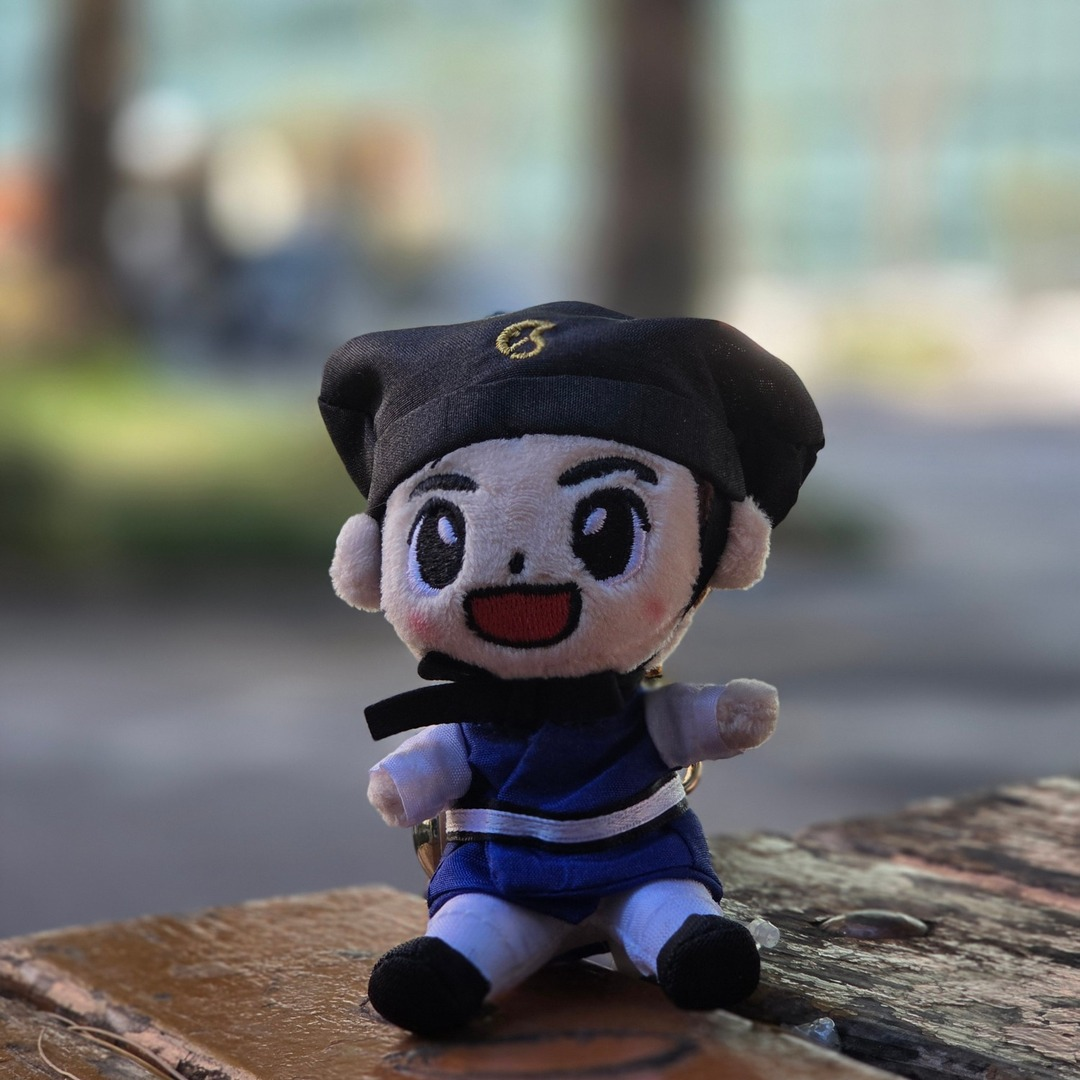
\includegraphics[width=0.325\columnwidth]{figures/fig_draft_final_gap_final.jpg}};
      \begin{scope}[x={(im.south east)}, y={(im.north west)}]
        \draw[orange, line width=0.8pt] (0.15,0.6435) rectangle (0.65,0.8102);
      \end{scope}
    \end{tikzpicture} \tabularnewline[1pt]
    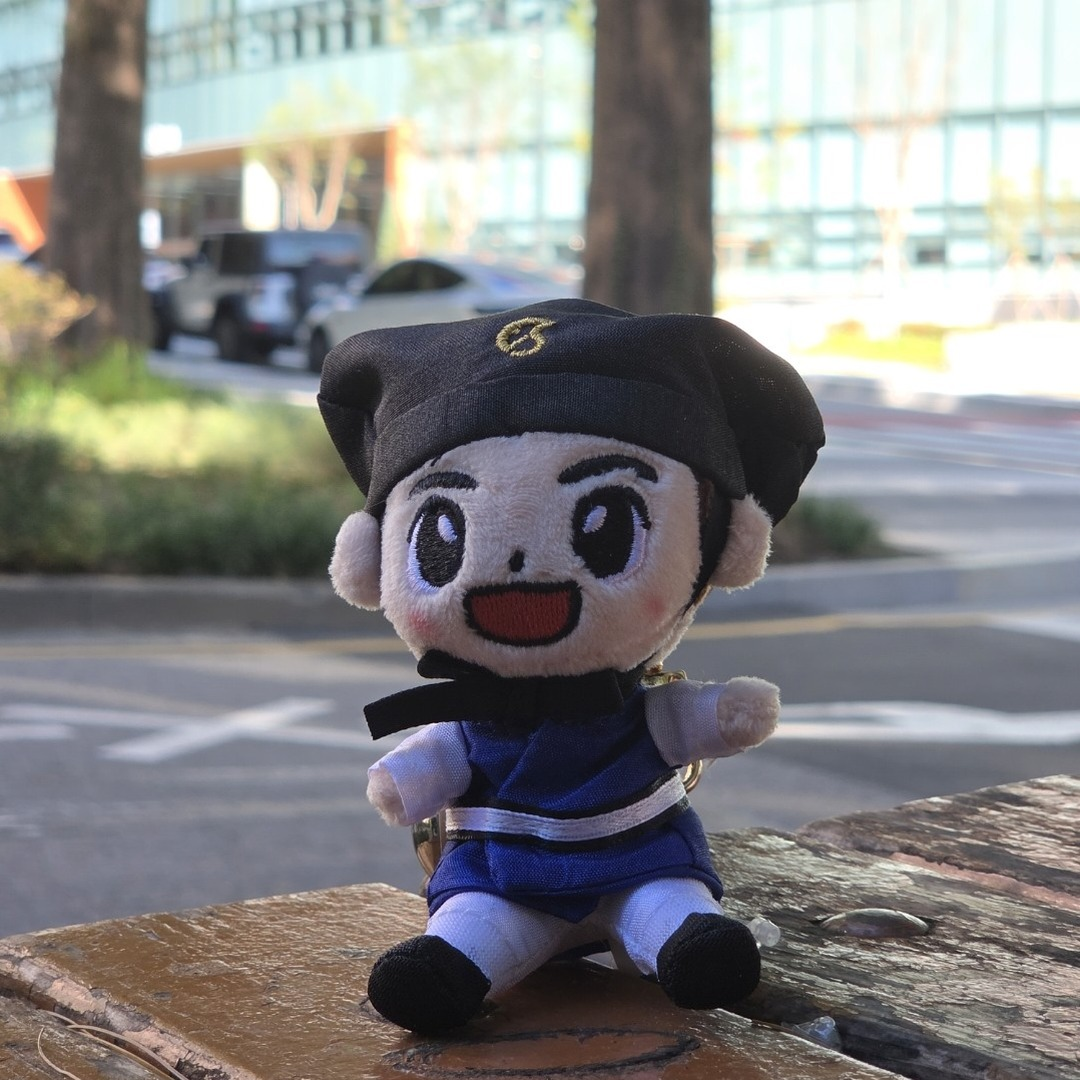
\includegraphics[width=0.325\columnwidth, trim=162 695 378 205, clip]{figures/fig_draft_final_gap_draft.jpg} &
    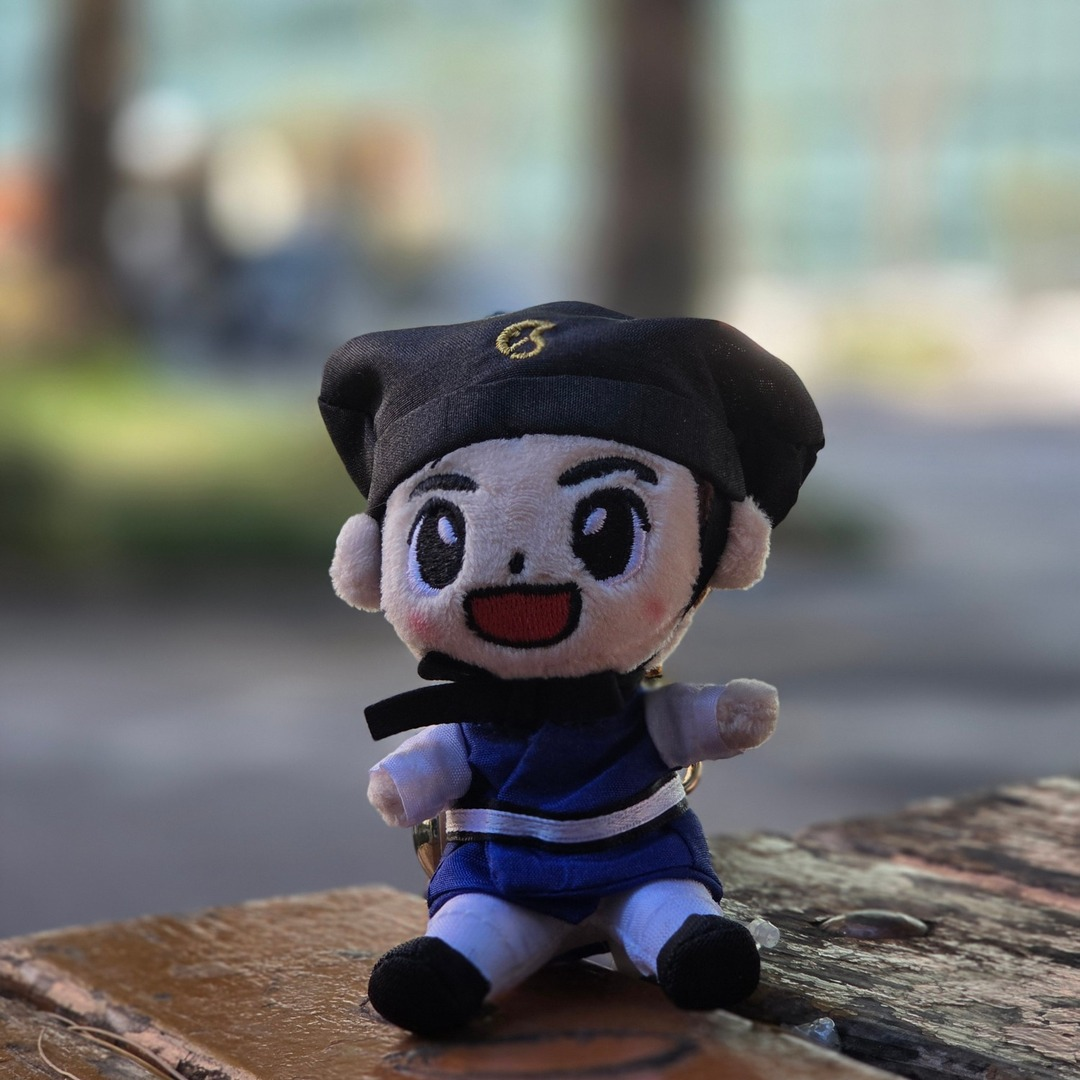
\includegraphics[width=0.325\columnwidth, trim=162 695 378 205, clip]{figures/fig_draft_final_gap_final.jpg} &
    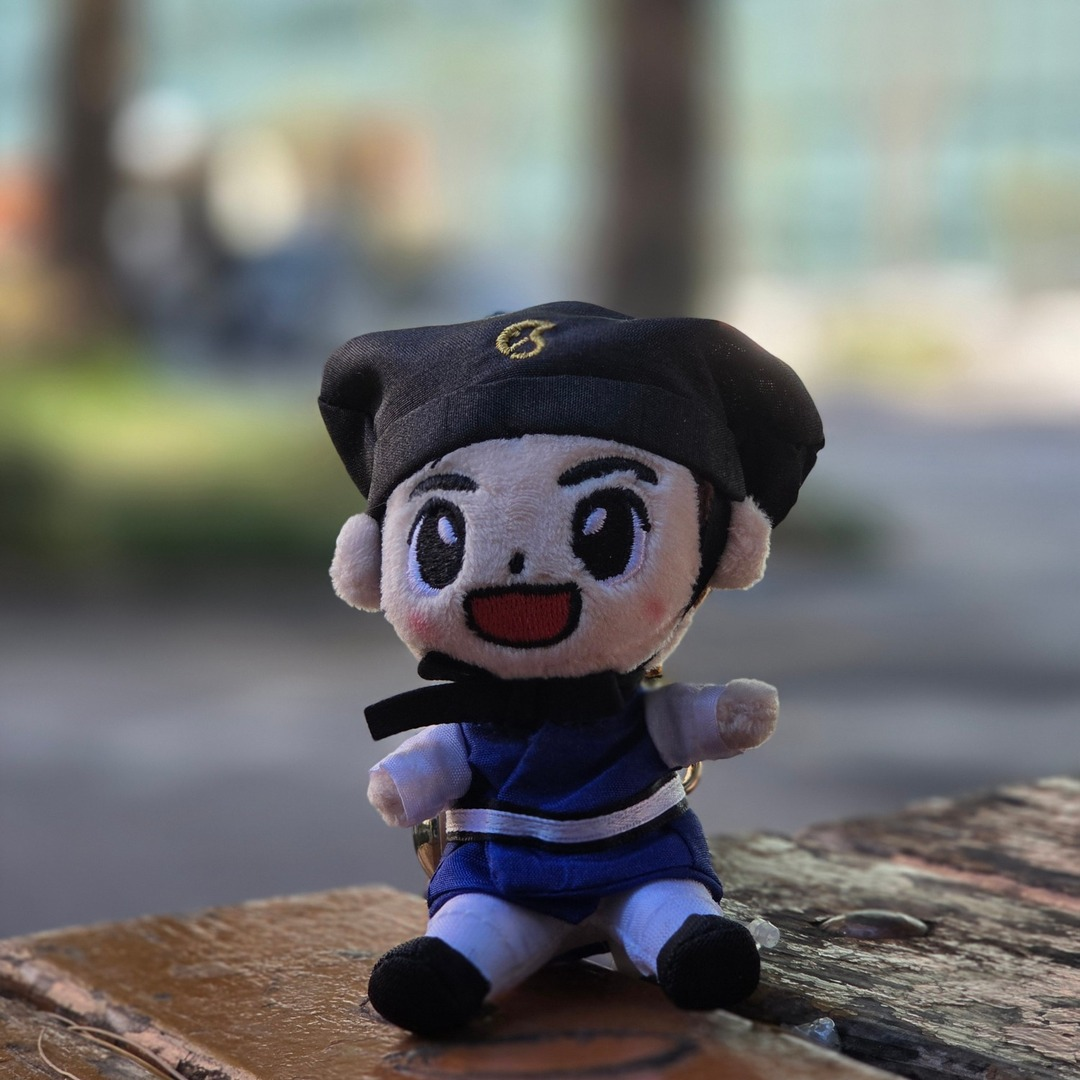
\includegraphics[width=0.325\columnwidth, trim=162 695 378 205, clip]{figures/fig_draft_final_gap_final.jpg}
    \tabularnewline[2pt]
    \parbox[t]{0.325\columnwidth}{\centering\scriptsize (a) Draft image} &
    \makebox[0.325\columnwidth][c]{%
      \parbox[t]{0.41\columnwidth}{\centering\scriptsize
        (b) Draft image with \\lightweight multi-frame composition}} &
    \parbox[t]{0.325\columnwidth}{\centering\scriptsize (c) Final image}
  \end{tabular}
  \caption{Draft--final visual differences in Portrait mode.}
  \label{fig:draft-final-gap}
\end{figure}



\subsection{Camera Usability}
\label{sec:camera-usability}
\label{sec:draft-background}

To enhance camera usability, Samsung aims to provide users with draft images as quickly as possible, support rapid consecutive captures, and minimize the visual difference between draft and final images.
To achieve these goals, Samsung employs a draft sequence, parallel capture, and lightweight multi-frame composition, respectively.

\myparagraph{Draft Sequence}
The draft sequence produces a draft image that users can view before computationally intensive post-processing generates the final image.
Once post-processing completes, the final image replaces the draft image.
To maintain responsiveness, Samsung delays final image generation until the camera application moves to the background in certain shot modes.
Consequently, users may view the draft image for an extended period, making it important to minimize the visual difference between draft and final images.

\myparagraph{Parallel Capture}
Parallel capture reduces the shot-to-shot interval by allowing a new capture request to be accepted before the preceding capture produces its draft image.
This is enabled by a capture-availability signal, \texttt{captureAvailable}, sent from the hardware abstraction layer (HAL) through the camera framework to the application.
By allowing consecutive captures to overlap, parallel capture enables users to take multiple photos in quick succession.

\myparagraph{Lightweight Multi-Frame Composition}
To reduce the visual difference between draft and final images, Samsung developed lightweight multi-frame composition (MFC) for the draft sequence.
MFC combines information from multiple captured frames to improve the draft image before it is displayed to users.
This difference is particularly noticeable in Portrait mode, where the background remains relatively sharp in the original draft image (Figure~\ref{fig:draft-final-gap}(a)), whereas it is blurred in the final image (Figure~\ref{fig:draft-final-gap}(c)).
With MFC, the draft image (Figure~\ref{fig:draft-final-gap}(b)) exhibits background blur that more closely resembles the final image.

\subsection{Challenges in Enabling MFC}
\label{sec:capture-timeout-risk}
\label{sec:guard-limit}

Enabling MFC in the draft sequence under parallel capture has caused frequent Capture Timeout violations during pre-release validation.
Although parallel capture allows consecutive capture requests to overlap, their draft sequences execute sequentially on a single draft worker.
For each accepted capture request, the camera collects the required input frames and metadata before enqueueing the corresponding draft sequence. The sequence may then wait in the queue while the capture's timeout clock continues to run.
Figure~\ref{fig:overlap} illustrates how successive captures can have progressively less time to execute their draft sequences, even when all draft sequences take equally long.
In particular, capture $i+2$ exceeds its deadline because its draft sequence must wait for the preceding draft sequences to complete.
The additional processing required for MFC can further increase queueing delays and cause more Capture Timeout violations.
Consequently, Samsung has not deployed MFC in the draft sequence of commercial devices, including the Galaxy S26 series.


\begin{figure}[t]
  \centering
  \resizebox{\columnwidth}{!}{\begin{figure}[t]
  \centering
  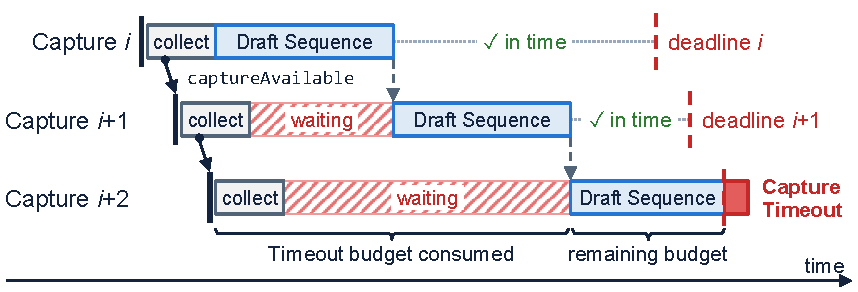
\includegraphics[width=\columnwidth]{figures/fig_parallel_capture_overlap.pdf}
  \caption{Capture Timeout caused by accumulated waiting time under parallel capture.}
  \label{fig:overlap}
\end{figure}

% % Notes: docs/exhibits.md#fig_parallel_capture_overlap
% \begin{tikzpicture}[font=\small,
%   collectstage/.style={draw=black!55, fill=gray!14},
%   draftstage/.style={draw=blue!45!black, fill=blue!14},
%   queued/.style={pattern=north east lines, pattern color=red!45, draw=red!35},
%   overrun/.style={draw=red!80!black, fill=red!65},
%   ddl/.style={red, dashed, thick},
%   sig/.style={->, black!75}]

%   \node[anchor=east] at (-0.2, 3.925) {capture $i$};
%   \draw[very thick] (0, 3.55) -- (0, 4.30);
%   \draw[collectstage] (0.05, 3.70) rectangle (0.90, 4.15);
%   \node at (0.475, 3.925) {\scriptsize collect};
%   \draw[draftstage] (0.90, 3.70) rectangle (3.50, 4.15);
%   \node at (2.20, 3.925) {\scriptsize Draft Sequence};

%   \draw[densely dotted, gray] (3.50, 3.925) -- (7.30, 3.925);
%   \node[fill=white, inner sep=1.5pt] at (5.40, 3.925)
%     {\footnotesize\textcolor{green!45!black}{\ding{51} in time}};
%   \draw[ddl] (7.30, 3.55) -- (7.30, 4.30);
%   \node[red, anchor=east] at (9.00, 3.925) {deadline $i$};

%   \fill[black!60] (0.35, 3.68) circle (1.3pt);
%   \draw[sig] (0.35, 3.66) -- (0.50, 3.17);
%   \node[anchor=west, black!75] at (0.42, 3.42)
%     {\scriptsize\texttt{captureAvailable}};

%   \node[anchor=east] at (0.3, 2.725) {capture $i{+}1$};
%   \draw[very thick] (0.50, 2.35) -- (0.50, 3.10);
%   \draw[collectstage] (0.55, 2.50) rectangle (1.40, 2.95);
%   \node at (0.975, 2.725) {\scriptsize collect};
%   \draw[queued] (1.40, 2.50) rectangle (3.50, 2.95);
%   \node[fill=white, inner sep=1.5pt] at (2.45, 2.725)
%     {\footnotesize\textcolor{red!60!black}{waiting}};
%   \draw[draftstage] (3.50, 2.50) rectangle (6.10, 2.95);
%   \node at (4.80, 2.725) {\scriptsize Draft Sequence};

%   \draw[densely dotted, gray] (6.10, 2.725) -- (7.80, 2.725);
%   \node[fill=white, inner sep=1.5pt] at (6.95, 2.725)
%     {\footnotesize\textcolor{green!45!black}{\ding{51} in time}};
%   \draw[ddl] (7.80, 2.35) -- (7.80, 3.10);
%   \node[red, anchor=east] at (10.00, 2.725) {deadline $i+1$};

%   \fill[black!60] (0.85, 2.48) circle (1.3pt);
%   \draw[sig] (0.85, 2.46) -- (1.00, 1.97);

%   \node[anchor=east] at (0.8, 1.525) {capture $i{+}2$};
%   \draw[very thick] (1.00, 1.15) -- (1.00, 1.90);
%   \draw[collectstage] (1.05, 1.30) rectangle (1.90, 1.75);
%   \node at (1.475, 1.525) {\scriptsize collect};
%   \draw[queued] (1.90, 1.30) rectangle (6.10, 1.75);
%   \node[fill=white, inner sep=1.5pt] at (4.00, 1.525)
%     {\footnotesize\textcolor{red!60!black}{waiting}};
%   \draw[draftstage] (6.10, 1.30) rectangle (8.70, 1.75);

%   \draw[overrun] (8.30, 1.30) rectangle (8.70, 1.75);
%   \node at (7.20, 1.525) {\scriptsize Draft Sequence};
%   \draw[ddl] (8.30, 1.15) -- (8.30, 1.90);
%   \node[red!70!black, anchor=west, align=left] at (8.80, 1.525)
%     {\footnotesize\bfseries Capture\\[-2pt]\footnotesize\bfseries Timeout};

%   \draw[dashed, gray, ->] (3.50, 3.67) -- (3.50, 2.98);
%   \draw[dashed, gray, ->] (6.10, 2.47) -- (6.10, 1.78);

%   \draw[decorate, decoration={brace, mirror, amplitude=4pt}]
%     (1.00, 1.10) -- (6.10, 1.10);
%   \node[anchor=north] at (3.55, 0.88) {\footnotesize Timeout budget consumed};
%   \draw[decorate, decoration={brace, mirror, amplitude=4pt}]
%     (6.10, 1.10) -- (8.30, 1.10);
%   \node[anchor=north] at (7.20, 0.88) {\footnotesize remaining budget};

%   \draw[->] (-1.3, 0.42) -- (9.7, 0.42) node[anchor=south east] {time};

% \end{tikzpicture}
}
  \caption{Capture Timeout caused by accumulated waiting time under parallel capture.}
  \label{fig:overlap}
\end{figure}

\myparagraph{Existing Strategy}
Even without MFC, Capture Timeout violations can occur under parallel capture, particularly on less powerful Samsung devices.
Because the camera framework is shared across device models, Samsung uses a common static thermal guard rather than introducing model-specific safeguards.
The guard skips optional image-processing stages (e.g., filter and watermark processing) in the draft sequence when the overheat level reaches 4 or higher.
Samsung's overheat level is a thermal indicator ranging from 0 to 6, with higher levels indicating stronger throttling.
However, the thermal guard cannot reliably determine whether additional processing, including MFC, can complete within a capture's remaining timeout budget based solely on the overheat level.

\myparagraph{Motivating Experiment}
To investigate whether adding MFC to the deployed draft sequence causes Capture Timeout violations under parallel capture, we conducted an experiment on the Galaxy S26 Ultra in Portrait mode.
We compared three draft configurations: \(S\), representing the currently deployed configuration with optional image-processing stages (e.g., filter and watermark processing); \(M+S\), which adds MFC \((M)\) to \(S\); and \(M\), which enables MFC without \(S\).
All three configurations retain the same mandatory encoding and saving stages.
We disabled the thermal guard so that the configured optional stages could execute even at overheat level~4 or higher, allowing us to examine timeout behavior across different thermal conditions.
We varied capture resolution (12MP and 24MP), memory conditions (normal and memory pressure), and starting overheat levels (0--6), resulting in 28 experimental settings.
For each configuration and setting, we conducted ten trials of up to 30 consecutive captures.
Table~\ref{tab:timeout_index} reports the earliest capture number at which a Capture Timeout occurred across the ten trials for \(M+S\) and \(M\), with a dash indicating no observed timeout within 30 captures.
The \(S\)-only results are summarized in the table note.

% Notes: docs/exhibits.md#tab_timeout_index
\providecolor{tmoS1}{RGB}{252,227,220}
\providecolor{tmoS2}{RGB}{239,160,140}
\providecolor{tmoS3}{RGB}{201,80,63}
\providecolor{tmoS4}{RGB}{143,36,32}

\newcolumntype{H}{>{\centering\arraybackslash}m{1.20cm}}
\newcolumntype{P}{>{\centering\arraybackslash}m{0.67cm}}

\providecommand{\tmoFirst}[2]{\cellcolor{#1}\makebox[\linewidth][r]{#2\hspace{1pt}}}
\providecommand{\tmoFirstW}[2]{\cellcolor{#1}\makebox[\linewidth][r]{\textcolor{white}{\textbf{#2}}\hspace{1pt}}}
\providecommand{\tmoNone}{\makebox[\linewidth][r]{--\hspace{1pt}}}

\begin{table}[t]
 \centering
 \caption{Earliest capture number with a Capture Timeout.}
 \label{tab:timeout_index}
 {\scriptsize\setlength{\tabcolsep}{1.3pt}%
 \begin{tabular}{@{}HPP|PP||PP|PP@{}}
 \toprule
 \multirow[c]{3}{=}[-10pt]{\makecell[c]{\textbf{Starting}\\\textbf{overheat}\\\textbf{level}}} &
 \multicolumn{4}{c||}{\raisebox{-3pt}{\textbf{Normal capture}}} &
 \multicolumn{4}{c@{}}{\raisebox{-3pt}{\textbf{Memory-pressure capture}}} \\[6pt]
 \cmidrule(lr){2-5}\cmidrule(l){6-9}
 &
 \multicolumn{2}{c|}{\raisebox{-3pt}{\textbf{12MP}}} &
 \multicolumn{2}{c||}{\raisebox{-3pt}{\textbf{24MP}}} &
 \multicolumn{2}{c|}{\raisebox{-3pt}{\textbf{12MP}}} &
 \multicolumn{2}{c@{}}{\raisebox{-3pt}{\textbf{24MP}}} \\[6pt]
 \cmidrule(lr){2-3}\cmidrule(lr){4-5}\cmidrule(lr){6-7}\cmidrule(l){8-9}
 & \raisebox{-2pt}{\textbf{M{+}S}} & \raisebox{-2pt}{\textbf{M}} &
 \raisebox{-2pt}{\textbf{M{+}S}} & \raisebox{-2pt}{\textbf{M}} &
 \raisebox{-2pt}{\textbf{M{+}S}} & \raisebox{-2pt}{\textbf{M}} &
 \raisebox{-2pt}{\textbf{M{+}S}} & \raisebox{-2pt}{\textbf{M}} \\[4pt]
 \midrule
 Lv0 &
 \tmoNone & \tmoNone & \tmoFirst{tmoS1}{29} & \tmoNone &
 \tmoNone & \tmoNone & \tmoFirst{tmoS1}{26} & \tmoNone \\
 Lv1 &
 \tmoNone & \tmoNone & \tmoFirst{tmoS1}{29} & \tmoNone &
 \tmoFirst{tmoS1}{24} & \tmoNone & \tmoFirst{tmoS2}{19} & \tmoNone \\
 Lv2 &
 \tmoFirst{tmoS1}{24} & \tmoNone &
 \tmoFirst{tmoS2}{18} & \tmoNone &
 \tmoFirst{tmoS2}{15} & \tmoFirst{tmoS1}{29} &
 \tmoFirst{tmoS2}{14} & \tmoFirst{tmoS1}{25} \\
 Lv3 &
 \tmoFirst{tmoS2}{13} & \tmoFirst{tmoS1}{21} &
 \tmoFirst{tmoS2}{12} & \tmoFirst{tmoS1}{20} &
 \tmoFirstW{tmoS3}{8} & \tmoFirst{tmoS2}{19} &
 \tmoFirstW{tmoS4}{5} & \tmoFirst{tmoS2}{13} \\
 \midrule
 Lv4 &
 \tmoFirstW{tmoS3}{8} & \tmoFirst{tmoS2}{16} &
 \tmoFirstW{tmoS3}{7} & \tmoFirst{tmoS2}{13} &
 \tmoFirstW{tmoS3}{6} & \tmoFirst{tmoS2}{13} &
 \tmoFirstW{tmoS4}{3} & \tmoFirstW{tmoS3}{7} \\
 Lv5 &
 \tmoFirstW{tmoS3}{8} & \tmoFirst{tmoS2}{12} &
 \tmoFirstW{tmoS3}{8} & \tmoFirst{tmoS2}{12} &
 \tmoFirstW{tmoS4}{4} & \tmoFirstW{tmoS3}{9} &
 \tmoFirstW{tmoS4}{4} & \tmoFirstW{tmoS3}{9} \\
 Lv6 &
 \tmoFirstW{tmoS3}{7} & \tmoFirst{tmoS2}{11} &
 \tmoFirstW{tmoS3}{7} & \tmoFirst{tmoS2}{11} &
 \tmoFirstW{tmoS4}{3} & \tmoFirstW{tmoS3}{6} &
 \tmoFirstW{tmoS4}{3} & \tmoFirstW{tmoS3}{6} \\
 \bottomrule
 \end{tabular}%
 }
 \par\vspace{3pt}
 {\scriptsize\begin{minipage}{0.933\columnwidth}
 \raggedright\setlength{\fboxsep}{1.8pt}%
 Earliest timeout capture number:~%
 \colorbox{tmoS1}{\strut\,${\geq}\,20$\,}%
 \colorbox{tmoS2}{\strut\,10--19\,}%
 \colorbox{tmoS3}{\strut\,\textcolor{white}{6--9}\,}%
 \colorbox{tmoS4}{\strut\,\textcolor{white}{${\leq}\,5$}\,}\par
 --: no timeout observed within 30 captures.\par
 \(S\)-only: no timeout observed in any of the 28 settings.\par
 \end{minipage}}
\end{table}

No Capture Timeout was observed with \(S\) alone across all 28 settings on the Galaxy S26 Ultra, although such violations can occur on less powerful Samsung devices. In contrast, adding MFC \((M+S)\) caused at least one timeout in 25 of the 28 settings, including 13 of the 16 settings starting below the thermal guard's level-4 cutoff.
This demonstrates that enabling MFC can cause frequent timeouts even when the initial overheat level is below the existing cutoff.
Conversely, all trials starting at level~4 or higher completed their first capture without a timeout, suggesting that the thermal guard may unnecessarily skip optional processing.
Moreover, even at the same starting overheat level, the earliest timeout occurred at different capture numbers depending on capture resolution, memory conditions, and draft configuration.
Executing \(M\) alone also increased the number of consecutive captures before the first Capture Timeout or avoided timeouts entirely within 30 captures, compared with \(M+S\).
These findings show that the number of consecutive captures that can safely complete is difficult to predict from the overheat level alone.
Therefore, the existing static thermal guard is insufficient for controlling MFC under parallel capture, motivating runtime control based on each capture's remaining timeout budget and processing workload.

\subsection{Goal}
\label{sec:research-goal}

Our goal is to reduce the visual gap between draft and final images by enabling MFC in the draft sequence under parallel capture while meeting each capture's Capture Timeout deadline.
Specifically, we aim to execute the optional stages---MFC (\(M\)) and existing image-processing stages (\(S\))---as often as possible without exceeding each capture's deadline.
Because draft sequences share a single worker, achieving this goal requires coordinating decisions on whether to execute these stages for each capture and when to allow the next capture request.
These decisions must also minimize delays between consecutive captures to preserve capture responsiveness.
